\section{Untersuchung gegebener Methoden (JEM)}

Da die beiden Bereiche des Requirements-Engineering und der Software-Architektur ein enormes Maß an Wissen und Fähigkeiten erfordern werden diese in der Regel von verschiedenen Teams betreut [8]. Wie bereits genannt, entstehen hier häufig Probleme durch fehlendes technisches Know-How über Software-Architektur spezifische Aspekte bei den Requirements-Engineers. Auch können diese oft nicht zwischen funktionalen Anforderungen (FR) und architekturspezifischen funktionalen Anforderungen (ASFR) unterscheiden [9]. ASFRs sind FRs welche kritisch, sehr risikobehaftet, volatil und bei Änderungen ein aufwendiges oder teures Refactoring mit sich bringen würden oder einen anderweitig großen Impakt auf die zu konzipierende Software-Architektur hätten [8]. Durch das fehlende Know-How entstehen unvollständige Anforderungs-Artefakte, in welchen wesentliche ASFRs für den Software-Architekten fehlen. \\

\begin{figure}[h]
	\centering
	\includegraphics[scale=0.5]{methoden.jpg} 
	\caption{Überblick über die untersuchten Methoden}\label{methoden}
\end{figure}

Sei ein vereinfachter Entwicklungsprozess wie in Abbildung \ref{methoden} gegeben. Zu sehen ist ein Kunde der eine System-Vision hat. Mit dieser Vision wendet er sich an einen Requirements Engineer, der einerseits über Gespräche und andererseits über seine Fähigkeiten versucht die System-Vision in Form von Anforderungen festzuhalten. Diese Anforderungen werden an den Software-Architekten weitergegeben, der wiederum versucht aus den Anforderungen einen Architekturentwurf zu generieren. Diesen Architekturentwurf wird er an die Entwickler weitergeben. Die Entwickler entwickeln dann das fertiggestellte System und liefern dies an den Kunden. In der Betrachtung der Zusammenarbeit zwischen Software-Architekt und Requirements Engineer sind vor allem die Punkte von Interesse, die vor der fertiggestellten Software-Architektur stehen. Somit sind als Stakeholder vor allem Kunde, Requirements Engineer und Software-Architekt von Bedeutung. Einfach formuliert soll es das Ziel sein die System-Vsion in einer korrekten Software-Architektur festzuhalten.\\

Im Folgenden sollen vier verschiedene Methoden untersucht werden, welche den Anspruch haben die Kluft in der Zusammenarbeit zwischen Software-Architekt und Requirements Engineer zu überbrücken. Dabei werden zunächst die Ziele der Methode herausgearbeitet und anschließend die Funktionsweise näher erläutert, bevor die vier Methoden im nachfolgenden Kapitel ausgewertet werden. Bei der Funktionsweise wird auf folgende Aspekte genauer eingegangen: \\

\begin{itemize}
\item \textit{Randbedingungen:} Gibt es Einschränkungen oder Vorbedingungen für die Ausführung der Methode?
\item \textit{Eingabe:} Welche Artefakte werden für die Ausführung der Methode benötigt?
\item \textit{Vorgehensmodell:} Wie wird die Methode durchgeführt?
\item \textit{Ausgabe:} Was liefert die Methode für ein Ergebnis? \\
\end{itemize}

\subsection{ADD 3.0 (FDD)}
\subsubsection{Beschreibung}
Attribut-driven-Design (ADD) bezeichnet ein Vorgehensmodell, bei dem iterativ ein Architekturdesign ausgearbeitet wird. ADD wird in Form von sogenannten Design Rounds durchgeführt. Eine Design-Round kann hierbei beispielsweise einem Sprint in SCRUM zugeordnet werden. Dies bedeutet in einem Projekt kann es mehrere Design-Rounds geben, mit denen die Software-Architektur verfeinert wird. \\

Eine Eigenschaft, die bei ADD besonders hervorsticht ist, dass es innerhalb der Design-Rounds eine klare Folge von Anweisungen gibt, die auszuführen sind um die Software-Architektur zu entwickeln. Hierbei ist relevant zu erwähnen, dass in ADD die Dokumentation und Analyse als wichtigste Elemente zur Entwicklung der Software-Architektur betrachtet werden. Nachteil bei ADD ist jedoch, dass die Voraussetzung hierfür ist, dass bereits primäre funktionale Anforderungen und Szenarien erhoben sind. Dies bedeutet ADD findet nicht direkt in der Anforderungsgewinnung Anwendung, sonder erst danach. Insgesamt umfasst ADD sieben Schritte die innerhalb einer Design-Round auszuführen sind.\\

Diese sind:
\begin{itemize}
\item[1:] Review Inputs
\item[2:] Establish Iteration goal by selecting drivers
\item[3:] Choose one or more elements of the system to refine
\item[4:] Choose one or more desing concepts that satisfy the selected drivers
\item[5:] Instantiate architectural elements, allocate responsiblities and define interfaces
\item[6:] Sketch views and record design decisions
\item[7:] Perform analysis of current design and review iteration goal and achievement of desing purpose
\end{itemize}
Um bei ADD eine Design-Round durchführen zu können sind jedoch zunächst einige Eingaben für den Prozess vorzubereiten.\\

Diese sind:
\begin{itemize}
\item Übergeordnete Zielstellung
\item Primäre funktionale Anforderungen
\item Szenarien
\item Einschränkungen
\end{itemize}

\paragraph{Step 1 - Überprüfung der Eingaben}
Zunächst muss sichergestellt werden, dass die übergeordnete Zielstellung für die darauffolgenden Design-Aktivitäten festgelegt ist. Diese kann beispielsweise die erstmalige Erstellung eines Design-Entwurfes oder die Verbesserung eines vorhandenen Architektur-Designs sein. Danach wird überprüft, ob die für die Design-Round relevanten Anforderungen und Szenarien korrekt sind. Hier ist unter anderem zu prüfen ob alle relevanten Stakeholder berücksichtigt werden und ob die erhobenen Anforderungen richtig priorisiert sind. Zuletzt muss noch geprüft werden, ob es Einschränkungen bezüglich der Software-Architektur gibt, die in der Design-Round zu berücksichtigen sind.\\

\paragraph{Step 2 - Festlegung des Ziels der Iteration durch Auswahl von Artefakten}
Eine Design-Runde 
\subsection{Probing (JEM)}

Das Ziel des Probing ist es, Requirements Engineers mit Fragen auszustatten die eine Erhebung architekturrelevanter Anforderungen, den ASFRs, ermöglichen. Diese Fragen werden Probing Questions (PQ) genannt. \\

\subsubsection{Ziele der Methode}

Die Haupttreiber architekturrelevanter Entscheidungen sind nicht-funktionale (NFR) bzw. qualitative Anforderungen [9]. Diese haben eine explizite Auswirkung auf die zu erstellende Architektur. Bei funktionalen Anforderungen bzw. ASFRs sind diese Auswirkungen meist implizit und müssen zunächst durch weitere Interviews mit dem Kunden herausgearbeitet werden. Auch sind hier die für einen Software-Architekten erforderlichen Informationen nicht immer klar in der Anforderung aufgeführt [9]. Dies kann zu falschen architektonischen Entscheidungen führen. Um dieses Problem anzugehen beschäftigen sich die Probing Questions mit den ASFRs. Requirements Engineers sollen mit Probing Questions ausgestattet werden um zusätzliche relevante Fragen stellen zu können. Dadurch soll während der Anforderungserhebung eine vollständigere Anforderungsspezifikation erstellt werden, in welcher die ASFRs aussagekräftiger sind [9]. Auch helfen diese den Requirements Engineers ein genaueres Verständnis für den Software-Architekten aufzubauen, welche Informationen er für die Konzeption und Implementierung der Software-Architektur benötigt. \\

\subsubsection{Funktionsweise der Methode}

Da das Probing eine Art Interview-Leitfaden bestehend aus PQs für die ausführlichere Extraktion von ASFRs und keinen methodischen Leitfaden für die Anwendung dieser zur Verfügung stellt, wird in den folgenden Paragraphen auf den Aufbau der PQs und nicht auf die Durchführung eines Interviews mit diesen eingegangen. \\

\paragraph{Randbedingungen}

Randbedingungen
Der REler muss gewillt sein, die PQs zu stellen...\\

\paragraph{Eingabe}

Eingabe


\paragraph{Vorgehensmodell}

Vorgehensmodell


TODO: PQ Kategorien und Typen aus (8). \\


TODO: NUR DIE ERSTEN BEIDEN SPALTEN ÜBERNEHMEN

\begin{table}[h] %h, t, b, p : here = genau an dieser Stelle, wenn möglich, top = für den Seitenanfang, bottom = für das Seitenende, p = für eine spezielle Seite mit Tabellen und Abbildungen
\caption{ASFR Kategorien und Beispiele}
\centering
\begin{tabular}{|p{3cm}|p{5cm}|}
%\begin{tabular}{|p{2cm}|p{4cm}|p{4cm}|p{6cm}|}%c, l, r, p{SIZEcm}, | : Zentrierter Text, linksbündiger Text, rechtsbündiger Text, Die Spalte soll SIZE cm breit sein, Das sog. Pipe-Symbol zeichnet einen senkrechten Strich zwischen die beiden Spalten
	\hline
	\textbf{ASFR Kategorie} & \textbf{Beschreibung} \\ %& \textbf{Beispiel ASFR} & \textbf{Beispiel Probing Question(s)} \\
	\hline
  	Audit Trail & Erleichtern der Auditierung der Systemausführung \\%& Das System muss jede Änderung an Kundendatensätzen für Auditzwecke erfassen. & - Müssen vor und nach Snapshots der Datenbank Tabellen gespeichert werden? \newline - Welche Art von Logs müssen geführt werden? \\
	\hline
\end{tabular}
\label{tab:asfr_category_table}
\end{table}


TODO: PQ-Flow aus (6). \\


\textbf{Paper so far:} \\
(6) Probing for Requirements Knowledge to Simulate Architectural Thinking \\
(8) What you see is what you get: Understanding Architecturally Significant Functional Requirements \\
(9) Identifying Architecturally Significant Functional Requirements \\


\paragraph{Ausgabe}

Ausgabe

\subsection{Component-Bus-System-Property (CBSP) (JEM)}\label{cbsp}
Component-Bus-System-Property, kurz CBSP, ist ein leichtgewichtiger Ansatz, um Anforderungen und Architektur mit Hilfe von Zwischenmodellen in \"ubereinstimmung zu bringen \cite{Gru01}. Dazu wird iterativ aus den Anforderungen ein CBSP Modell gebildet, welches Anforderungs- und Architektur-Modellelemente miteinander verkn\"upft. \\

\subsubsection{Ziele der Methode}

Der CBSP Ansatz hilft Software-Architekten dabei Architekturelemente wie Komponenten und Konnektoren, Architektur Eigenschaften, Abh\"angigkeiten zwischen diesen Elementen und passende Architekturstile zu finden. Dabei unterst\"utzt das CBSP den Software-Architekten dabei folgende Herausforderungen, um Anforderungen und Architektur in \"ubereinstimmung zu bringen, zu behandeln: \\

\begin{itemize}
\item \textit{\"uberbr\"uckung unterschiedlicher Formalit\"atsebenen}: Das Zwischenmodell von CBSP reduziert die Semantische L\"ucke zwischen meist informell in nat\"urlicher Sprache gehaltenen Anforderungen auf einer h\"oheren Abstraktionsebene und eher formell gehaltenen Architekturbeschreibungen \cite{Gru01}.
\item \textit{Modellierung nicht-funktionaler Anforderungen}: CBSP erm\"oglicht, die sonst schwere Modellierung von nicht-funktionalen Anforderungen als Architekturmodell sowohl auf der System- wie auch der Architekturebene \cite{Gru01}. 
\item \textit{Aufrechterhaltung evolution\"arer Konsistenz}: Aufrechterhaltung von Konsistenz und Nachverfolgbarkeit ist ein schwieriges Unterfangen, da eine einzelne Anforderung mehrere architektonische Anliegen betreffen kann und ein einzelnes Architekturelement typischerweise mehrere Beziehungen zu verschiedenen Anforderungen hat \cite{Gru01}. Diese Schwierigkeiten werden vom CBSP Zwischenmodell behoben.
\item \textit{Unvollst\"andige Modelle und iterative Entwicklung}: Das CBSP Zwischenmodell ben\"otigt auf Grund seines iterativen Vorgehensmodells keine von Beginn an vollst\"andige Anforderungsspezifikation. Desweiteren k\"onnen bestimmte Anforderungen erst vollst\"andig verstanden werden, wenn die Software-Architektur modelliert oder sogar partiell implementiert wurde \cite{Gru01}.
\item \textit{Gr\"o\ss{}e und Komplexit\"at Behandeln}: Gro\ss{}systeme m\"ussen meist hunderte bis tausende von Anforderungen erf\"ullen. Da CBSP sich in jeder Iteration nur mit einem Teil der architektonisch relevanten Anforderungen besch\"aftigt kann es diese Komplexit\"at beherschen und den Fokus erh\"ohen. Jede Aktivit\"at von CBSP befasst sich mit der Filterung von Anforderungen oder dem Zusammenfassen mehrerer Anforderungen in eine \cite{Gru01}.
\item \textit{Verschiedene Stakeholder mit unterschiedlichen Interessen}: Anforderungen und Architektur in Einklang zu bringen ist auch ein Prozess, in welchem heterogene Stakeholder mit widerspr\"uchlichen Zielen, Erwartungen und Terminologien involviert sind. CBSP versucht hier die richtige Balance zwischen diesen abweichenden Interessen zu finden indem es wichtige Stakeholder involviert \cite{Gru01}. \\
\end{itemize}

Um bei der Bew\"altigung dieser Herausforderungen zu unterst\"utzen bietet das CBSP: \\

\begin{itemize}
\item einen leichtgewichtigen Ansatz Anforderungen zu verfeinern durch die Bereitstellung eines kleinen erweiterbaren Sets von Architektur Schl\"usselkomponenten, 
\item einen Mechanismus um die Anzahl relevanter Anforderungen zu reduzieren und auf die relevantesten ASFRs zu fokussieren, 
\item Beteiligung von wichtigen Stakeholdern, 
\item einen regulierbaren Voting-Mechanismus um Konflikte und unterschiedliche Auffassungen zwischen Architekten zu beheben und
\item Toolunterst\"utzung f\"ur bestimmte Schritte des Ansatzes \cite{Gru01}. \\
\end{itemize}

\subsubsection{Funktionsweise der Methode}

Das CBSP erweitert, wie in Abbildung \ref{fig_cbsp_model} zu sehen ist, den Gedanken des Twin-Peaks Modells. Das Zwischenmodell des CBSP verkn\"upft die Anforderungen mit der Architektur. Das iterative Vorgehen kann dabei sogar auf verschiedenen Detail- bzw. Abstraktionsstufen angewandt werden \cite{Gru01}. 
Um das Vorgehen genauer verstehen zu k\"onnen wird zun\"achst die Taxonomie des CBSP betrachtet. \\

\begin{figure}[h]
	\centering
	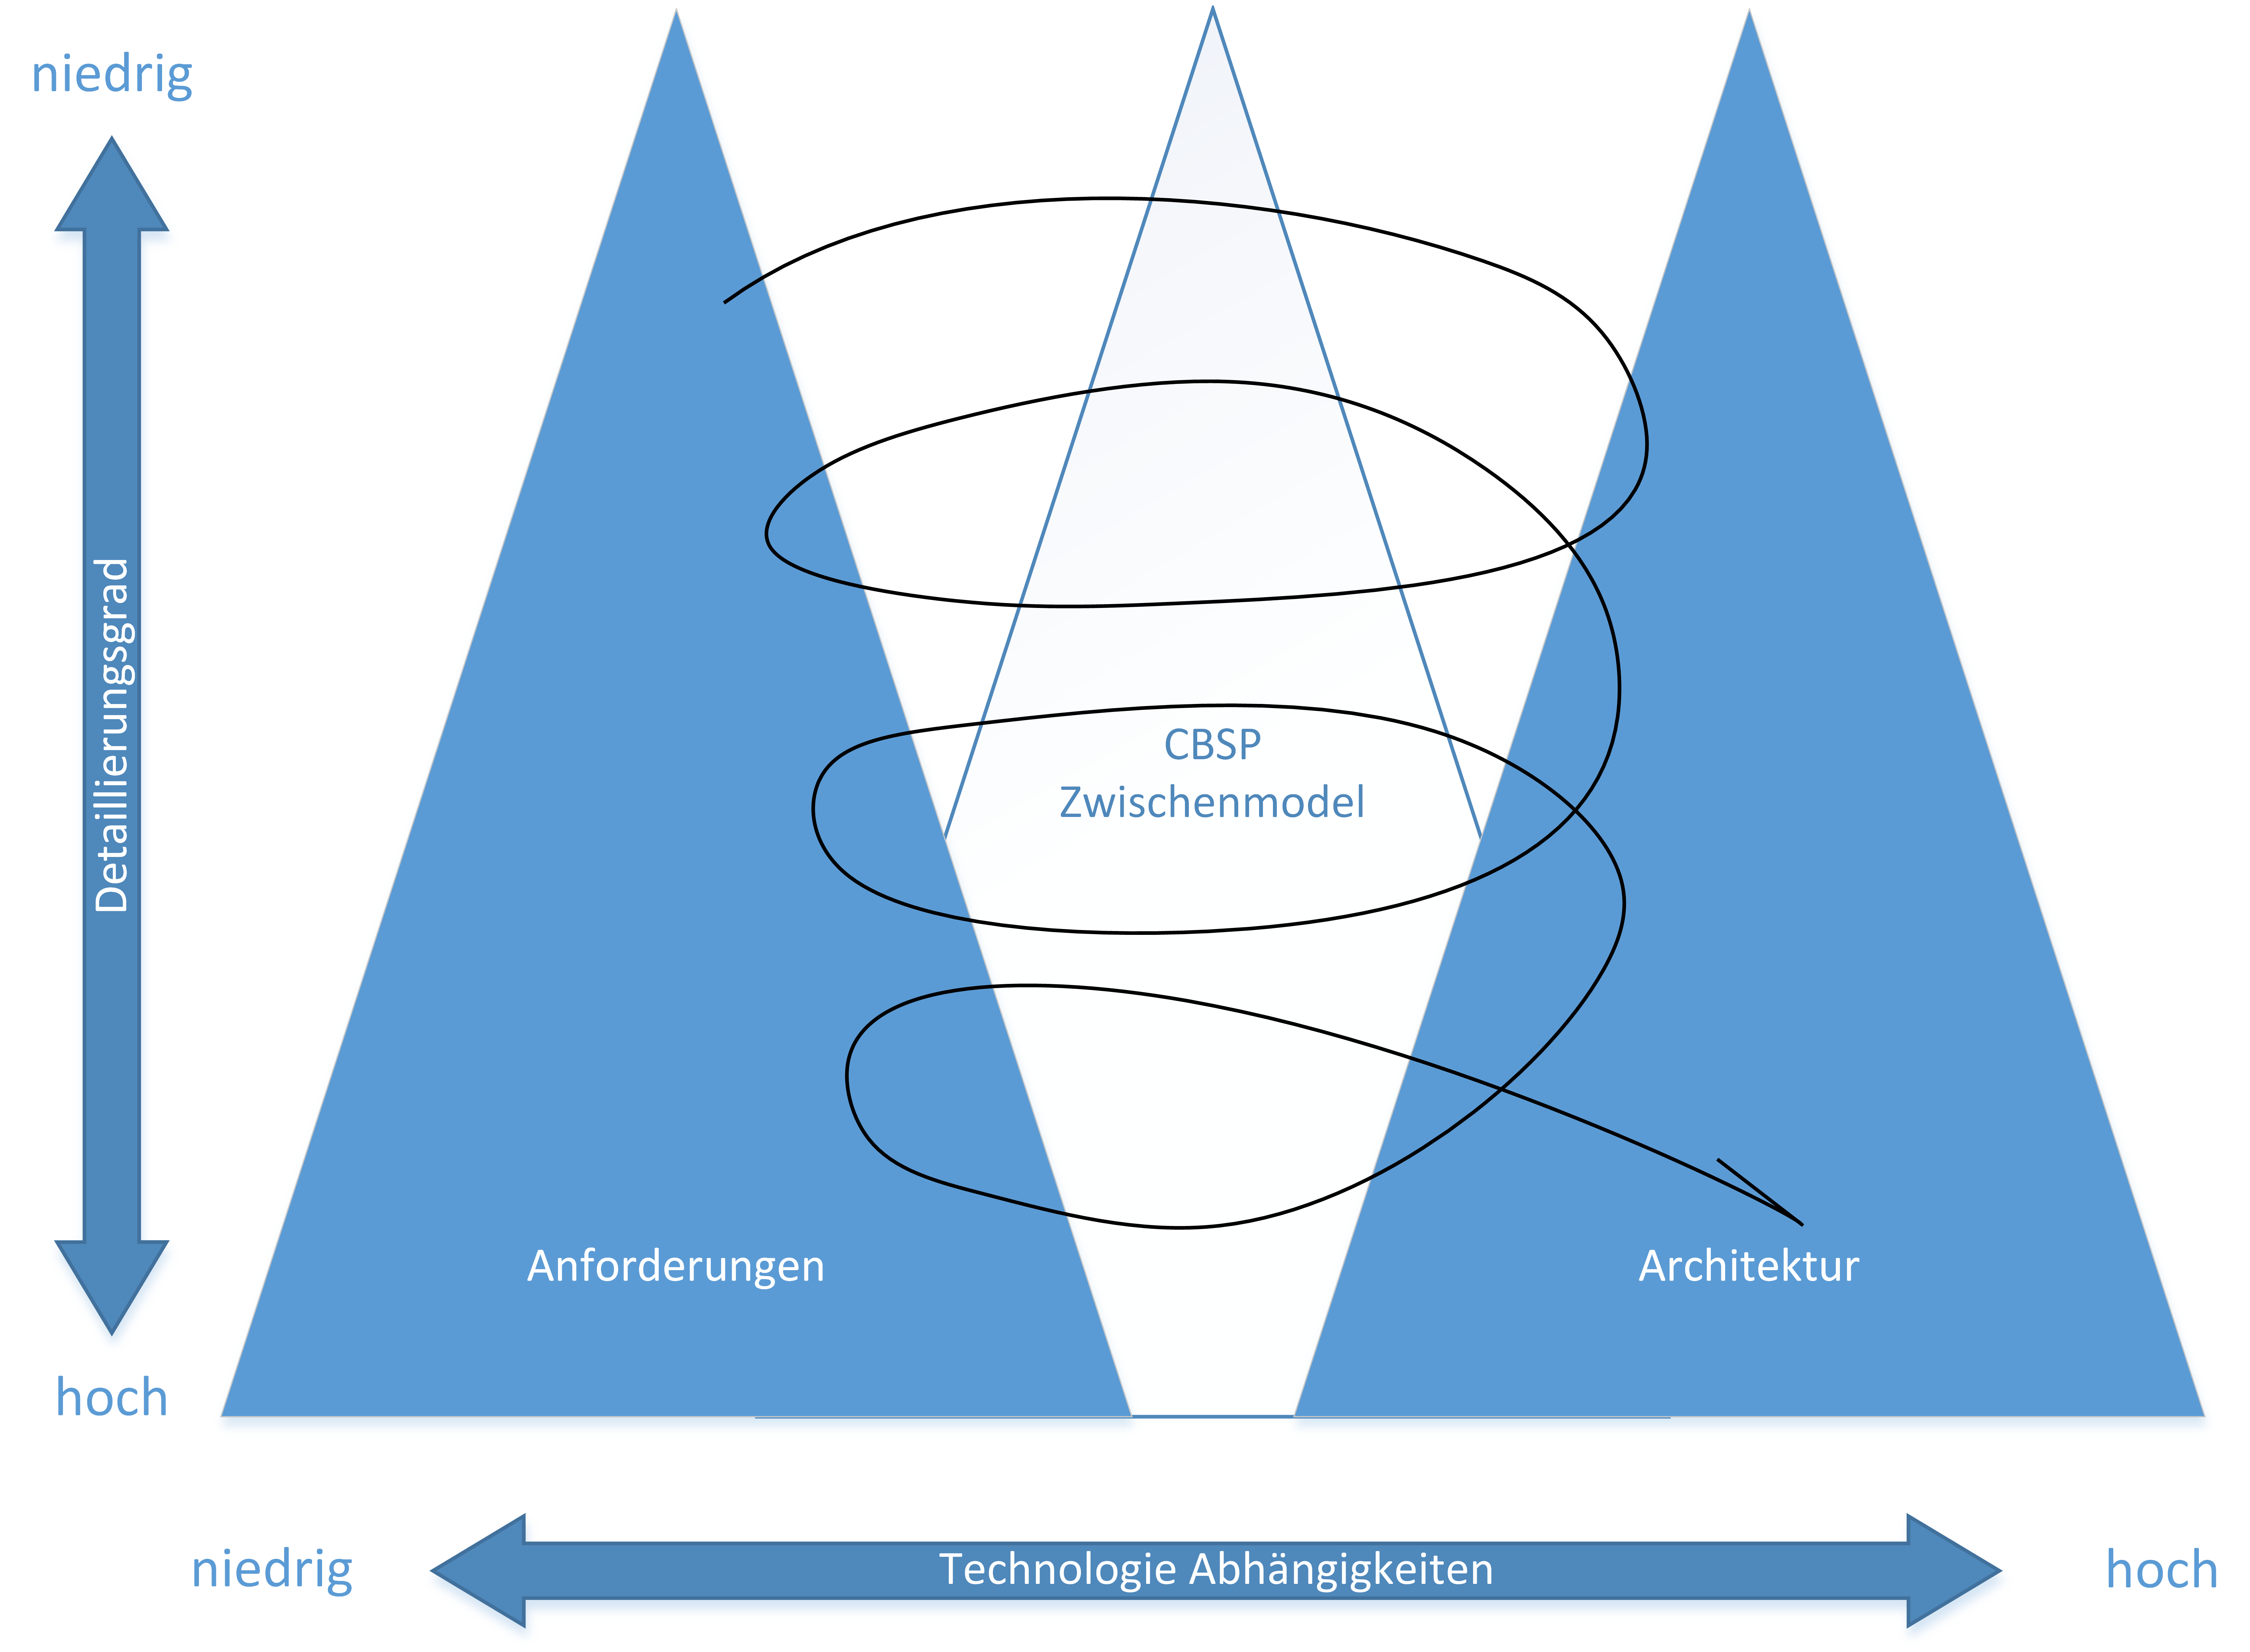
\includegraphics[scale=0.5]{cbsp_model2.png} 
	\caption{CBSP Modell Kontext \cite{Gru01}}
	\label{fig_cbsp_model}
\end{figure}

\emph{CBSP Taxonomie:}
Das Metamodell von CBSP beinhaltet die Basiskonstrukte einer Architektur und ist in sechs Dimensionen aufgeteilt: \\

\begin{itemize}
\item[1.] \textit{C}: sind Elemente, welche individuelle Komponenten der Software-Architektur beschreiben oder involvieren. Diese sind in Datenkomponenten (C\textsubscript{D}) und Verarbeitungskomponenten (C\textsubscript{P}) unterteilt. So k\"onnte beispielsweise die Anforderung: \\
	\textit{R: Benutzern das direkte manipulieren von Kalkulationstabellen erlauben.} \\
	in folgende CBSP Modellelemente verfeinert werden: \\
	\textit{C\textsubscript{P}: UI Komponente f\"ur Kalkulationstabellen Manipulation.} \\
	\textit{C\textsubscript{D}: Daten f\"ur Kalkulationstabellen.}  \cite{Gru01}
\item[2.] \textit{B}: sind Elemente, welche Konnektoren beschreiben. Zum Beispiel: \\
	\textit{R: Manipulierte Daten in Kalkulationstabellen muss im Dateisystem gespeichert werden.} \\
	kann in folgendes CBSP Modellelement verfeinert werden: \\
	\textit{B: Konnektor der die Interaktion zwischen UI und Persistenz-Komponenten erm\"oglicht.} \cite{Gru01}
\item[3.] \textit{S}: sind Elemente, welche systemweite Features beschreiben oder solche, die zu einer gr\"o\ss{}eren Untermenge von Komponenten und Konnektoren passen. Zum Beispiel: \\
	\textit{R: Der Benutzer soll angemessene Filter und Visualisierungen ausw\"ahlen k\"onnen.} \\
	kann in folgendes CBSP Modellelement verfeinert werden: \\
	\textit{S: Das System soll eine strikte Trennung von Datenhaltungs-, -Bearbeitungs- und -Visualisierungs-Komponenten vornehmen.} \cite{Gru01}
\item[4.] \textit{CP}: sind Elemente, welche Eigenschaften, wie Zuverl\"assigkeit, Portabilit\"at, Skalierbarkeit, Anpassbarkeit und Erweiterbarkeit, von Daten- oder Verarbeitungskomponenten beschreiben. Zum Beispiel: \\
	\textit{R: Das Benutzer soll die Daten entfernt mit minimale wahrgenommener Latenz visualisieren k\"onnen.} \\
	kann in folgendes CBSP Modellelement verfeinert werden: \\
	\textit{CP: Die Datenvisualisierungs-Komponente soll effizient sein und inkrementelle Updates unterst\"utzen.} \cite{Gru01}
\item[5.] \textit{BP}: sind Elemente, welche Eigenschaften von Konnektoren beschreiben. Zum Beispiel: \\
	\textit{R: Updates f\"ur Systemfunktionen sollen mit minimaler Ausfallzeit m\"oglich sein.} \\
	kann in folgendes CBSP Modellelement verfeinert werden: \\
	\textit{BP: Robuste Konnektoren sollen zur Verf\"ugung gestellt werden, um das Hinzuf\"ugen und Entfernen von Laufzeitkomponenten zu erleichtern.} \cite{Gru01}
\item[6.] \textit{SP}: sind Elemente, welche systemweite Eigenschaften bzw. Eigenschaften von Subsystemen beschreiben. Zum Beispiel: \\
	\textit{R: Die Daten der Kalkulationstabellen m\"ussen verschl\"usselt werden bevor sie \"uber das Netzwerk versandt werden.} \\
	kann in folgendes CBSP Modellelement verfeinert werden: \\
	\textit{SP: Das System soll sicher sein.} \cite{Gru01} \\
\end{itemize}

Aus diesen Elementen wird das CBSP Zwischenmodell aufgebaut. Das Metamodell zu diesen Elementen ist in Abbildung \ref{fig_cbsp_meta_model} dargestellt. Jedes CBSP Artefakt beschreibt eine architekturrelevantes Anliegen und beschreibt eine fr\"uhe Architekturentscheidung des zu erstellenden Systems \cite{Gru01}. \\

Von einer Anforderung zu einem CBSP Element kann eine Verfeinerung, siehe Beispiel (5), oder Generalisierung, siehe Beispiel (6), erfolgen. Diese beiden m\"oglichen Anpassungen basieren auf Notwendigkeiten, welche durch bestimmte Eigenschaften des zu erstellenden Systems, Charakteristika der Anwendungsdom\"ane oder Hintergrund und Erfahrung des Software-Architekten, erwachsen \cite{Gru01}. Da es f\"ur Verfeinerung und Generalisierung keine allgemeinen formalen Regeln gibt, ist es h\"aufig notwendig hierf\"ur den Kunden bzw. weitere Stakeholder wie den Requirements Engineer zu konsultieren \cite{Gru01}. 

\begin{figure}[h]
	\centering
	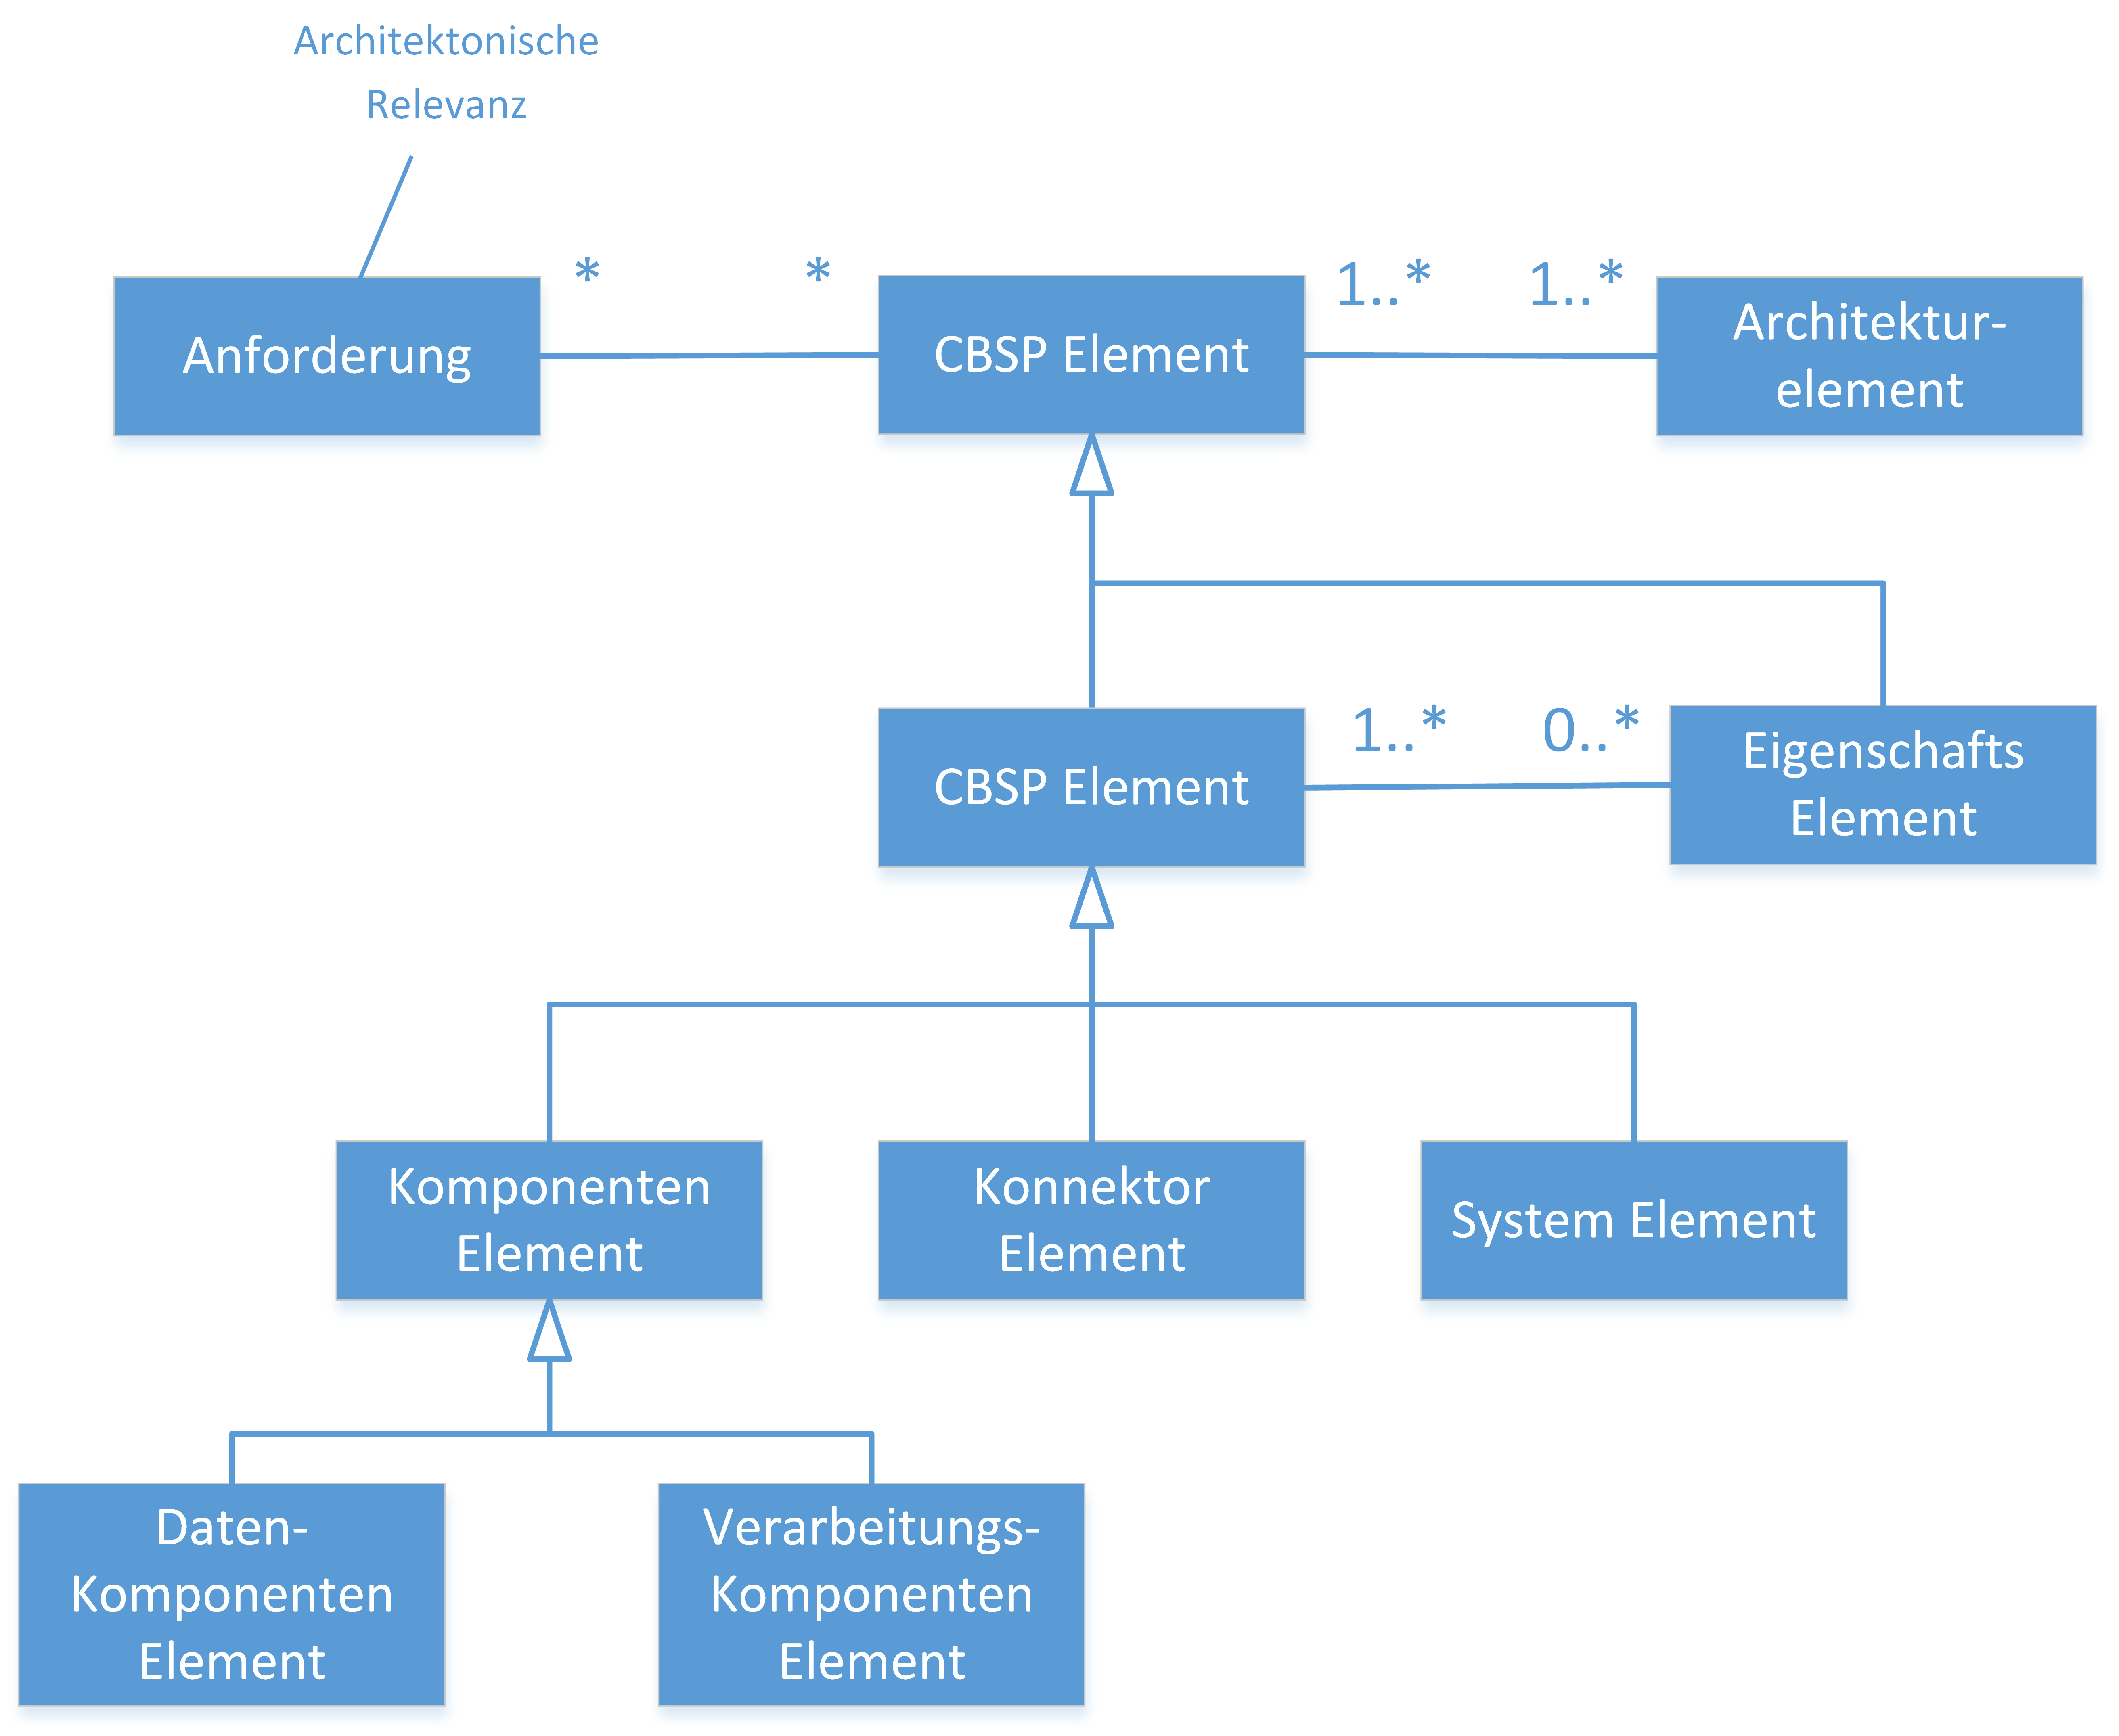
\includegraphics[scale=0.6]{cbsp_meta_model.png} 
	\caption{CBSP Metamodell \cite{Gru01}}
	\label{fig_cbsp_meta_model}
\end{figure}

\paragraph{Randbedingungen}

Damit CBSP erfolgreich angewandt werden kann muss die Bereitschaft zur Mitarbeit aller involvierten Stakeholder gegeben sein. In fast allen Schritten k\"onnen diese bei Unklarheiten oder f\"ur Feedback herangezogen werden. In einigen Schritten ist deren Mitarbeit verpflichtend. \\
Desweiteren m\"ussen die Software-Architekten \"uber ein gewisses Mindestma\ss{} an Erfahrung und Wissen verf\"ugen um die einzelnen Schritte kompetent durchf\"uhren zu k\"onnen. Daf\"ur gibt es allerdings keine Liste mit Mindestvoraussetzungen oder ein Minimum an Jahren an Berufserfahrung. Hier muss klar sein ob der Architekt die n\"otigen Kompetenzen besitzt um wichtige Entscheidungen selbstst\"andig treffen zu k\"onnen. \\

\paragraph{Eingabe}

Als Eingabe ben\"otigt das CBSP eine erste Anforderungsspezifikation. Diese muss noch nicht vollst\"andig sein, denn sie kann in jeder Iteration weiter erg\"anzt werden. Da CBSP nicht auf FRs oder NFRs zugeschnitten ist, werden alle Anforderungen genutzt, denn beide Anforderungstypen haben sowohl explizit als auch implizit Informationen, welche f\"ur die Software-Architektur relevant sind \cite{Gru01}. \\


\paragraph{Vorgehensmodell} 
Jede Iteration von CBSP besteht aus f\"unf Schritten, welche im folgenden vorgestellt werden. \\

\emph{Schritt 1: Auswahl der Anforderungen f\"ur die n\"achste Iteration} - 
Um die Komplexit\"at zu reduzieren werden hier, wie bereits angesprochen, durch ein Team von Architekten nur Anforderungen f\"ur die Iteration ausgew\"ahlt, welche mittels zweier Kriterien durch den Requirements Engineer als wichtig oder durchf\"uhrbar bewertet wurden: (1) die \textit{Bedeutung} zeigt die Relevanz und den Wert f\"ur den Projekterfolg, (2) w\"ahrend die \textit{Durchf\"uhrbarkeit} technische, \"okonomische und politische Bedingungen ber\"ucksichtigt \cite{Gru01}. Diese Anforderungen k\"onnen formell, informell oder semi-formell notiert sein. \\

\emph{Schritt 2: Architektonische Klassifizierung der Anforderungen} - 
In Schritt zwei klassifizieren die Software-Architekten die selektierten Anforderungen mit Hilfe der CBSP Taxonomie. Desweiteren werden alle so klassifizierten Anforderungen in einer Tabelle anhand ihrer Relevanz zu den sechs CBSP Dimensionen bewertet. Die Bewertung erfolgt \"uber eine Ordinalskala (nicht=0; partiell=1; weitgehend=2; voll=3) und beschreibt die Auswirkung, welche die Anforderung auf eine oder mehrere der jeweiligen CBSP Elemente hat \cite{Gru01}. Eine Beispielhafte Bewertung der Anforderungen \textit{R01: Unterschiedliche Ladungstypen unterst\"utzen}, \textit{R02: Verschiedene Fahrzeuge unterst\"utzen} und \textit{R09: Sch\"atzung der Frachtankunft und Fahrzeugverf\"ugbarkeit unterst\"utzen} ist Tabelle \ref{tab:relevance_profiles} zu entnehmen \cite{Gru01}. 

\begin{table}[h] %h, t, b, p : here = genau an dieser Stelle, wenn m\"oglich, top = f\"ur den Seitenanfang, bottom = f\"ur das Seitenende, p = f\"ur eine spezielle Seite mit Tabellen und Abbildungen
\caption{Beispiel Relevanzprofile nach \cite{Gru01}}
\centering
\begin{tabular}{|l|c|c|c|c|c|c|}
\hline 
\textbf{Anforderungen} & \textbf{C} & \textbf{B} & \textbf{S} & \textbf{CP} & \textbf{BP} & \textbf{SP} \\ 
\hline 
R01 & 1,33 & 0,33 & \cellcolor{Gray} 1,67 & 1,00 & 0,33 & 0,33 \\ 
\hline 
R02 & \cellcolor{Gray} 2,00 & 0,00 & 1,00 & 1,33 & 0,00 & 0,00 \\ 
\hline 
R09 & \cellcolor{Gray} 2,67 & 1,33 & 2,00 & 0,33 & 0,00 & 0,00 \\ 
\hline 
\end{tabular} 
\label{tab:relevance_profiles}
\end{table}

\begin{table*}[t] %h, t, b, p : here = genau an dieser Stelle, wenn m\"oglich, top = f\"ur den Seitenanfang, bottom = f\"ur das Seitenende, p = f\"ur eine spezielle Seite mit Tabellen und Abbildungen
\caption{CBSP zu Architekturstil Mapping nach \cite{Gru01}}
\centering
\newcolumntype{M}[1]{>{\centering\arraybackslash}p{#1cm}}
\begin{tabular}{|p{3cm}|p{4,2cm}|M{2}|M{1}|M{2}|M{1,5}|M{1,3}|}%{|l|c|c|c|c|c|c|} 15
\hline 
\textbf{CBSP Dimensionen} & \textbf{Eigenschaften} & \textbf{Client-Server} & \textbf{C2} & \textbf{Event-basiert} & \textbf{Schichten-Architektur} & \textbf{Pipes und Filter} \\ 
\hline 
Datenkomponente & aggregiert & ++ & ++ & ++ & + & - \\ 
 & persistent & ++ & o & o & o & o \\ 
 & gestreamt & - & - & - & - & + \\ 
 & gecached & ++ & + & - & - & - \\ 
\hline 
Verarbeitungskomponente & Dienste anbieten / Nur konsumieren & ++ & o & o & o & o \\ 
 & hat N Schnittstellen & ++ & + & ++ & - & - \\ 
 & stateful & + & ++ & ++ & + & - \\ 
 & lose gekoppelt & + & + & ++ & - & ++ \\ 
 & kann migriert werden & + & ++ & ++ & - & - \\ 
\hline 
Konnektor & synchron & ++ & - & + & ++ & - \\ 
 & asynchron & - & ++ & ++ & - & ++ \\ 
 & lokal & - & ++ & o & ++ & + \\ 
 & verteilt & ++ & ++ & ++ & - & + \\ 
 & sicher & + & o & o & + & o \\ 
\hline 
(Sub-)System & effizient & o & + & + & o & - \\ 
 & skalierbar & + & o & - & - & + \\ 
 & weiterentwickelbar & ++ & ++ & ++ & - & ++ \\ 
 & portierbar & o & + & o & ++ & o \\ 
 & zuverl\"assig & o & o & - & o & o \\ 
 & dynamisch & + & ++ & ++ & - & ++ \\
\hline 
\end{tabular} 
\label{tab:cbsp_to_style_mapping}
\end{table*}

\emph{Schritt 3: Identifizierung und Aufl\"osung von falschen Zuordnungen bei der Klassifizierung} - 
Da mehrere Software-Architekten diese Klassifizierung unabh\"angig voneinander vornehmen, m\"ussen im dritten Schritt m\"ogliche Abweichungen aufgedeckt, diskutiert und behoben werden. Dies ist wichtig um Missverst\"andnisse, mehrdeutige Anforderungen, implizites Wissen, und widerspr\"uchliche Auffassungen zu identifizieren und Risiken bei der Verfeinerung der Anforderungen zu reduzieren \cite{Gru01}. Bei der Diskussion k\"onnen auch der Kunde und Requirements Engineer involviert sein. Der erarbeitete Konsens sorgt f\"ur ein einheitliches Verst\"andnis der Anforderungen und die Relevanz dieser f\"ur die Software-Architektur. Wenn keine Unstimmigkeiten mehr vorliegen werden die Anforderungen weiter ausged\"unnt indem alle Anforderungen, welche eine geringere Relevanz haben als ein vorher definierter Wert der Ordinalskala, wie beispielsweise "weitgehend", vorerst verworfen werden. Dabei wird auf Abh\"angigkeiten zwischen den Anforderungen geachtet um kritische nicht zu verwerfen. Alle akzeptierten Anforderungen werden inklusive gesammelter Probleme und Unklarheiten in den n\"achsten Schritt \"ubernommen. \\

\emph{Schritt 4: Architektonische Verfeinerung der Anforderungen} - 
Im vorletzten Schritt werden die CBSP Elemente umformuliert oder aufgeteilt, welche \"uberlappende CBSP Dimensionen und architektonische Anliegen aufweisen. Wenn ein CBSP Element beispielsweise weitgehend Komponenten-relevant, voll Konnektor-relevant und weitgehend Konnektor-Eigenschafts-relevant ist, erh\"oht es das Verst\"andnis und die Pr\"azision wenn es in mehrere Architekturentscheidungen, verk\"orpert als CBSP Element, aufgesplittet wird. Ein einzelnes CBSP Artefakt kann w\"ahrend diesem Prozess mehrfach als Nebenprodukt bei verschiedenen Anforderungen auftauchen, w\"ahrend diese Redundanzen identifiziert und eliminiert werden \cite{Gru01}. \\

In diesem Schritt gibt es zwei Varianten welche entweder einzeln oder sogar kombiniert ausgef\"uhrt werden k\"onnen. Variante eins betrachtet zun\"achst nur die gro\ss{}en strukturellen Aspekte des Systems (C, B und S Elemente). Dies hat den Vorteil, dass der Architekt leichter einen Überblick behalten kann, da die beiden Aspekte (Struktur und Funktionalit\"at vs. nicht-funktionale Eigenschaften) separat betrachtet werden. Die Eigenschaften der drei Elemente werden in einem gesonderten (Sub-)Prozess identifiziert. Die zweite Variante identifiziert in einem Schritt sowohl die strukturellen Elemente als auch ihre nicht-funktionalen Eigenschaften. Der Vorteil hierbei ist, dass der Software-Architekt sich auf ein kompletten System Aspekt (oder eine kleine Menge von Aspekten) konzentrieren kann. \\

\emph{Schritt 5: Abgleich der Entscheidungen zwischen Architekturelementen und -stilen mit CBSP} - 
Wenn alle ausgew\"ahlten Anforderungen im CBSP Model modelliert wurden, sodass keine Konflikte zwischen Software-Architekt und Requirements Engineer bestehen und alle CBSP Modellelementen weitgehend relevant zu einer der sechs CBSP Dimensionen sind, kann in Schritt f\"unf ein erster Architektur-Prototyp abgeleitet werden. \\
Die Bestimmung eines passenden Architekturstiles mit den zu den CBSP Modellelementen passenden Architekturmustern ist nicht immer einfach. Zum einen existiert kein formaler Ansatz f\"ur diesen Prozess, zum anderen k\"onnen mehrere Architekturstile zum generierten CBSP Modell passen. F\"ur diese Aufgabe gibt es verschiedene Verfahren. Hier wird die Selektion eines passenden Architekturstiles mit Hilfe einer Matrix aufgestellt, siehe Tabelle \ref{tab:cbsp_to_style_mapping}. Diese Metrix stellt die CBSP Dimensionen mit geeigneten Eigenschaften potentiellen Architekturmustern gegen\"uber. Allerdings ist diese Tabelle nicht vollst\"andig, denn weitere Eigenschaften f\"ur die CBSP Elemente sind denkbar und es werden auch nicht alle existierenden Architekturstile angeboten. Zum einen ist sie daf\"ur nicht gedacht, sie soll lediglich eine Hilfestellung bei der Wahl eines passenden Architekturstils bieten sobald mehr als einer passend erscheint. Daf\"ur muss sie nur so umfassend wie eben n\"otig sein. Zum anderen w\"urde eine vollst\"andige Tabelle \textit{jedes} Softwaresystem darstellen und nicht auf eine konkrete Dom\"ane zurecht geschnitten sein. Au\ss{}erdem w\"are eine solche unm\"oglich zu erstellen \cite{Gru01}. Die endg\"ultige Wahl liegt allerdings beim Software-Architekten. \\

Anschlie\ss{}end muss der Software-Architekt die CBSP Modellelemente in entsprechende Architekturelemente wie Komponenten, Konnektoren, Konfigurationen, Pakete und Daten mit den gew\"unschten Eigenschaften umwandeln \cite{Gru01}. \\

\paragraph{Ausgabe}

Nach der Ausf\"uhrung der f\"unf Schritte und mehrfachen Iterationen sollte eine Software-Architektur gegeben sein, welche die selektierten Anforderungen zu einem m\"oglichst hohen Grad erf\"ullt.

%\textbf{Paper Cites:} \\
%(\cite{Gru01}) Reconciling software requirements and architectures with intermediate models \\


%Viel ^^ (Weaving the Software Development Process Between Requirements and Architectures)

%RE und SA sind sehr voneinander abh\"angig (Descending the twin Peaks)


%\begin{itemize}
%\item[1.] Text
%\item[2.] Text
%\item[3.] Text \\
%\end{itemize}
\subsection{sCenario and gOal based SysteM develOpment methoD (COSMOD) (FDD)}\label{scgo}
COSMOD-Requirements Engineering (COSMOD-RE) beschreibt ein iteratives Vorgehen zum gleichzeitigen Design von Anforderungen und Software-Architektur. Kerngedanke bei COSMOD-RE ist eine Aufteilung in vier Hierarchiestufen, wo sowohl Architektur als auch Anforderungen definiert werden. In diesen vier Hierarchiestufen wird einerseits aus der Anforderungssicht und andererseits aus der Architektursicht betrachtet, welche Anforderungen und Komponenten dem System zuzuordnen sind.
\subsubsection{Ziele der Methode}
Kernziel von COSMOD-RE ist es die Entwicklung von Anforderungs- und Architekturartefakten für softwareintensive eingebettete Systeme zu unterstützen. Ein Ziel- und Szenario-basierter Ansatz wie COSMOD-RE, der das Co-Design von Architekturartefakten und Anforderungen ermöglicht muss jedoch einige Anforderungen erfüllen um einen Nutzen zu haben. Die Anforderungen an eine solchen Methodik sind \cite{pohl}\\
 
\begin{itemize}
\item Parallele Entwicklung von Anforderungen und Architekturartefakten \\
Da Anforderungen und die Software Architektur die Kerntreiber hinter innovativen Projekten sind ist es wichtig beide gleichermaßen zu nutzen, sodass keines von beiden in den Vordergrund tritt \cite{pohl}.
\item Unterstützung der Anordnung von Anforderungen und Architekturartefakten \\
Werden Anforderungen und Architekturartefakte parallel entwickelt kann es passieren, dass Inkonsistenzen auftreten. Um diese zu vermeiden ist es notwendig, dass COSMOD-RE diese erkennt und behebt \cite{pohl}.
\item Definition detaillierter Anforderungen auf der Basis von Architekturartefakten \\
Ohne technisches Wissen fällt es Stakeholdern schwer notwendige Details für die Erhebung architekturrelevanter Anforderungen zu liefern. Daher sollte es COSMOD-RE ermöglichen die detaillierten Anforderungen erst nach der initialen Definition von Architekturartefakten zu liefern \cite{pohl}. 
\item Nutzung einer Abstraktionshierarchie \\
Da bei einem Co-Design Vorgehen eine große Komplexität bestehen kann ist es notwendig eine Abstraktionshierarchie einzuführen um diese entsprechend zu behandeln \cite{pohl}.\\
\end{itemize}

\subsubsection{Funktionsweise der Methode}
Das wichtigste Element von COSMOD-RE ist die Abstraktionshierarchie. Über diese werden alle Aktivitäten die im Rahmen der Methodik stattfinden eingeordnet und miteinander in einen Kontext gesetzt. So wird auf jeder Ebene der Abstraktionshierarchie eine Architektursicht und eine Anforderungssicht erzeugt. Hierbei ist jedoch zu beachten, dass bei COSMOD-RE nicht unbedingt ein Top-Down-Ansatz zu wählen ist, da Anforderungsartefakte und Architekturartefakte auf allen Ebenen gleichzeitig bearbeitet werden können.\\

\paragraph{Randbedingungen}
Bei der Anwendung von COSMOD-RE ist zu beachten, dass einige Bedingungen erfüllt sein müssen um die Methodik richtig anzuwenden:\\

\begin{itemize}
\item Definition einer Abstraktionshierarchie \\
Es gibt keine Richtlinien bezüglich der Definition der Abstraktionshierarchie. Dies bedeutet, dass die verwendeten Hierarchiestufen im jedem Projekt neu festgelegt werden müssen. Ferner ist hierbei von Relevanz, zu definieren, wo die Trennlinien zwischen verschiedenen Abstraktionsstufen sind \cite{sikora}.
\item Verknüpfung von Anforderungs- und Architekturmodellen \\
Da im Rahmen von COSMOD-RE Anforderungsartefakte und Architekturartefakte parallel entwickelt werden ist es notwendig diese miteinander zu verknüpfen um sie in den Kontext des Ziels der Software zu bringen. Für diese Verknüpfung ist die Anwendung von Methodenfragmenten notwendig \cite{sikora}.
\item Definition von Konsistenzbedingungen \\
Für die Definition von Konsistenzbedingungen gibt es keinen allgemeingültigen Ansatz. Daher ist es notwendig in jedem Projekt neu zu definieren, ob Konsistenz gegeben ist oder nicht \cite{sikora}.\\
\end{itemize}

Sind diese Randbedingungen geklärt ist es möglich COSMOD-RE anzuwenden.\\

\paragraph{Eingabe}

\paragraph{Vorgehensmodell}
\paragraph{Ausgabe}

\subsubsection{Beschreibung}
In der Anforderungserhebung soll es m\"oglich sein Anforderungen in einer Form zu erheben, die es Software Architekten einfacher macht, den Architekturentwurf zu konzipieren. Um dies zu realisieren bietet sich eine Kombination aus Ziel-basierten Ans\"atzen und Szenario-basierten Ans\"atzen an. Die Kombination ist deswegen von Relevanz, weil ein Ansatz allein nicht ausreichen kann um die Anforderungen in angemessener Weise zu erheben.\\

\subsubsection{Ziel-basierte Ans\"atze}
Ziel-basierte Ans\"atze zielen vorrangig darauf ab, ein umfassendes Verst\"andnis der W\"unsche und Ziele der Stakeholder sowie auf die zu erzielenden Auswirkungen auf die Systemumgebung ab (Silkora Referenz S.18). Dies bedeutet, dass es bei Ziel-basierten Ans\"atzen vor allem darauf ankommt, zu verstehen, welche Vision der Stakeholder von dem Zuk\"unftigen System hat. Bei der Erfassung dieser Vision ist ein nat\"urlichsprachlicher Ansatz fehlerbehaftet, da hier sehr aufw\"andige manuelle Konsistenzpr\"ufungen notwendig w\"aren. Deswegen bieten sich hier vor allem Modell-basierte Ans\"atze an.\\

Ein gutes Beispiel f\"ur ein Modell-basierten Ansatz ist der KAOS-Ansatz. Dieser Ansatz bietet den Vorteil, dass er mit wenigen pr\"azise formulierten Modellierungsobjekten auskommt. Dies ist deswegen ein Vorteil, weil so kein besonders tief reichendes Fachwissen notwendig ist um das Modell zu interpretieren. Ferner ist der Ansatz f\"ur die Konzeption softwareintensiver eingebetteter Systeme geeignet, was eine verzahnte Entwicklung von Anforderungen und Architektur \"uber mehrere Abstraktionsstufen hinweg erm\"oglicht (Silkora Referenz S.31).\\

\paragraph{KAOS}
Lamsweerde (Lamsweerde Referenz) beschreibt eine modellbasierten Ansatz zur Darstellung von Zielen und den Referenzen innerhalb von Zielen. Hierf\"ur muss zun\"achst eine genauere Betrachtung der Zieldefinition vorgenommen werden. So sind in dem Kontext der KAOS-Methode Ziele in Bahavioral-Goals und Soft-Goals zu unterteilen. \\

Behavioral-Goals beschreiben eine deklarative Sicht auf Ziele, die beschreibt, wie ein System sich zu verhalten hat. Dies bedeutet, dass in diesem Fall besonders das Verhalten von Systemen im Fokus steht. G\"ultig ist eine endliche Menge von Verhaltensweisen des Systems. \\

Grunds\"atzlich lassen sich Bahavioral-Goals in zwei Kategorien aufteilen, die Achive-Goals und die Maintain/Avoid-Goals. Die Achive-Goals beschreiben Systemverhalten, bei dem es darauf ankommt, dass ein System zu einem definierten Zeitpunkt einen definierten Zustand erreicht. Maintain/Avoid-Goals beschreiben Systemverhalten, bei dem es darauf ankommt, dass ein System \"uber einen definierten Zeitraum hinweg einen definierten Zustand aufrechterh\"alt, oder einen definierten Zustand vermeidet.\\

Soft-goals beschreiben Pr\"aferenzen innerhalb von g\"ultigen Systemverhaltensweisen. Diese lassen sich zun\"achst in funktionale Ziele und nicht funktionale Ziele aufteilen. Die funktionalen Ziele k\"onnen die folgenden Kategorien haben:
\begin{itemize}
\item Satisfaction: Funtionale Ziele, die sich damit besch\"aftigen User-Anfragen zu beantworten.
\item Information: Funtionale Ziele, die damit besch\"aftigt sind User \"uber wichtige Systemzust\"ande zu informieren.
\item Stim-response: Funktionale Ziele, die sich damit besch\"aftigen auf Events eine angemessene Reaktion zu erzeugen.
\end{itemize}
Mit dem gegebenen Ziel die Zusammenarbeit zwischen Requirements Engineer und Software Architekt zu optimieren sind vor allem die funktionalen Ziele der Soft-Goals und die Behavioral-Goals von Relevanz.\\

der KAOS Ansatz, der die zuvor beschriebenen Zielarten als Grundlage nutzt, verwendet zur Modellierung Und-/Oder-Graphen, die in diesem Kontext Zieldiagramm genannt werden. Jedes im Graphen modellierte Ziel wird zun\"achst durch eine Reihe von Eigenschaften in einer Zielschablone charakterisiert. Die Eigenschaften k\"onnen unter anderem Name, Definition, Quelle, Zielkategorie und Priorit\"at sein.\\

--TODO-- Erzeugung Abbildung Und-Oder-Graph + Beschreibung der Elemente\\

Das Problem von Ziel-basierten Ans\"atzen wie dem KAOS Ansatz ist, dass eine Software Architektur allein basierend auf den Zielen wichtige Aspekte vernachl\"assigt. So zum Beispiel welche Rolle diese Ziele erreichen soll und gegebenenfalls wie die dieses Ziel umzusetzen ist. Daher ist es notwendig Szenario-basierte Ans\"atze zu betrachten.\\

\subsubsection{Szenario-basierte Ans\"atze}
Szenario-basierte Ans\"atze zielen vorrangig darauf ab, die wesentlichen geforderten Interaktionen des Systems mit dessen Umgebung zu definieren und mit den Stakeholdern abzustimmen (Silkora Referenz S.18).\\

Um die optimale Zusammenarbeit zu st\"utzen ist es notwendig, die Szenarien in einer Kombination aus Anwendungsfalldiagrammen und Message Sequence Charts graphisch zu modellieren. Dadurch, kann der Zusammenhang zwischen Szenarien aufgezeigt werden und wichtige Aspekte, die von Bedeutung f\"ur den Design der Softwarearchitektur sind, ber\"ucksichtigt werden. Es ist mit diesem Vorgehen m\"oglich Szenarien zu komplexeren Szenarien zusammenzusetzen und des weiteren Iterationen und alternative Szenarienverl\"aufe abzubilden (Silkora Referenz S.33). Bei der Betrachtung von Szenarien ist es jedoch auch hier notwendig, diese zun\"achst in Schablonen zu dokumentieren, um eine pr\"azise Beschreibung zu haben. In einer Schablone soll unter anderem festgehalten werden, welche prim\"aren und sekund\"aren Akteure gegeben sind. Ferner sollen eine Kurzbeschreibung und mit dem Szenario verkn\"upfte Ziele gegeben sein, um klar hervorzuheben, in welchem Kontext das Szenario zu sehen ist.\\

\paragraph{Anwendungsfalldiagramm}
Das Anwendungsfalldiagramm zeigt eine \"Ubersicht \"uber die Anwendungsf\"alle eines Systems oder einer Systemkomponente. Es stellt zudem die Akteure des Systems (der Komponente) und deren Beteiligung an den Anwendungsf\"allen grafisch dar (Silkora Zitat S.34). \\

Anwendungsf\"alle k\"onnen als Oberbegriff f\"ur Szenarien betrachtet werden, da ein Szenario sich aus einem Anwendungsfall generieren l\"asst. Dies bedeutet ein Anwendungsfall kann Grundlage für eine Vielzahl von Szenarien sein. \\

--TODO-- Anwendungsfalldiagramm beispielabbildung mit Notationselementen\\

Zu den Notationselementen eines Anwendungsfalldiagramms z\"ahlen:
\begin{itemize}
\item Akteur: Als Akteur l\"asst sich eine Person oder Entit\"at bezeichnen, die mit dem zu konzipierenden System in Beziehung steht. Diese k\"onnen zum Beispiel Nutzer sein, die \"uber eine Eingabemaske Daten eintragen sollen.
\item Systemgrenze: Systemgrenzen umschlie\ss{}en das geplante System. Akteure, die mit dem System interagieren befinden sich au\ss{}erhalb der Systemgrenze, w\"ahrend die dem System zugeordneten Anwendungsf\"alle sich innerhalb der Systemgrenze befinden.
\item Anwendungsfall: Ein Anwendungsfall beschreibt eine Funktionalit\"at des geplanten Systems. In Kombination mit dem Akteur, der in Relation zu einem Anwendungsfall steht, wird dargestellt, was das System machen soll.
\item Erweiterung eines Anwendungsfalls: Ein Anwendungsfall kann mittels Include- oder Extend-Beziehung erweitert werden. Dies soll es erm\"oglichen komplexere Anwendungsf\"alle abzubilden und gleichzeitig die Anzahl der Redundanzen m\"oglichst gering halten. Eine Include-Beziehung bedeutet hierbei, dass ein Anwendungsfall einen weiteren Anwendungsfall beinhaltet. Die Extend-Beziehung bedeutet, dass es zu einem Anwendungsfall eine Erweiterung unter einer Bedingung gibt. Die Bedingung gibt an welche Konditionen erfüllt sein müssen dass die Erweiterung greift.
\end{itemize}
Anwendungsfalldiagramme stellen Akteure und Anwendungsfälle dar. Dadurch wird veranschaulicht welche Akteure mit welchen Anwendungsfällen in Beziehung stehen und ob es wichtige Beziehungen zwischen verschiedenen Anwendungsfällen gibt. Grundsätzlich ist es möglich Anwendungsfalldiagramme auf verschiedenen Abstraktionsstufen abzubilden um so sowohl für das Gesamtsystem, als auch für die Teilsysteme die Beziehungen zu betrachten. Um jedoch Szenarien präzise zu spezifizieren reichen Anwendungsfalldiagramme nicht aus.\\

\paragraph{Message-Sequence-Charts}
Mithilfe von Message-Sequence-Charts ist es möglich eine präzise Spezifikation der verschiedenen Szenarien eines Anwendungsfalls zu generieren (Silkora Zitat S.37). Bei der Betrachtung der Zusammenarbeit zwischen Software-Architekt und Requirements-Engineer ist zunächst nur eine Teilmenge der Notationselemente der Message-Sequence-Charts relevant. Wichtigster Aspekt der Message-Sequence-Charts ist, dass diese vor allem die Akteure und ihre Interaktionen mit dem System hervorheben.\\

Grundsätzlich werde in einem Message-Sequence-Chart Nachrichten und Instanzen abgebildet. Eine Instanz kann hierbei z.B. ein System oder ein Akteur sein. Als Nachricht wird im Kontext der Message-Sequence-Charts der Austausch einer Information bezeichnet. Dies können z.B. Signale oder Daten sein, die zwischen den Instanzen versendet werden (Silkora Referenz S.38). \\

--TODO-- Abbildung zu MSC und Beschreibung\\

Neben den einfachen Message-Sequence-Charts gibt es High-Level-Message-Sequence-Charts (HLMSC), die es ermöglichen eine Komposition mehrerer Message-Sequence-Charts zu bilden und so komplexere Zusammenhänge darzustellen. Grundsätzlich besteht ein HLMSC aus einem Start- und Endknoten, einem oder mehreren Verweisknoten und einer Menge von Kanten. Die Start- und Endknoten dienen hierbei der Begrenzung des Anwendungsfalls.  Die Verweisknoten sind als Verweise zu einfachen Message-Sequence-Charts oder weiteren HLMSC zu sehen. Ungerichtete Kanten dienen der Darstellung der Komposition und mithilfe von gerichteten Kanten lässt sich Iteration darstellen.\\

--TODO-- Abbildung zu HLMSC \\

Wenn Anwendungsfälle in Kompositionen zusammengefasst werden lässt sich argumentieren, dass man bei hinreichenden Kompositionen in den Bereich der Ziele gelangt. Somit wird deutlich, dass der Szenario-basierte Ansatze implizit schon eine Betrachtung der Ziele fordert.\\

\subsubsection{Kombination der Ans\"atze}
Wenn die wesentlichen Ziele der Stakeholder bekannt sind, besteht die M\"oglichkeit, diejenige Architekturalternative auszuw\"ahlen, mit der die Ziele am besten erf\"ullt werden k\"onnen (Silkora Referenz S.18).\\

Sowohl Ziel-basierte Ansätze als auch Szenario-basierte Ansätze sind alleinstehend nicht ausreichend, um eine Grundlage für einen guten Architekturansatz auf der Basis von Anforderungen zu generieren. Hierfür ist es notwendig, die Ansätze zu kombinieren. \\

Ein Beispiel für eine solche Kombination ist der COSMOD-RE (sCenario and gOal based SysteM develOpment methoD) Ansatz. \\

\paragraph{COSMOD-RE}

\begin{itemize}
\item[1] System: Die Systemebene beschreibt die oberste Ebene, bei der in der Anforderungssicht das System als ganzes betrachtet wird. Im Fokus stehen dabei die Interaktionen mit dem System. Weiter werden funktionale Anforderungen und Qualitätsanforderungen erstellt, die sich auf das Gesamtsystem beziehen. Die Architektursicht konzentriert sich hier auf die Definition von externen Systemschnittstellen. Hier definierte Artefakte sollen primär die Kommunikation mit Stakeholdern unterstützen.
\item[2] Komponenten: Die Komponentenebene bezeichnet die Aufteilung des Systems in einzelne Komponenten aus denen sich dieses zusammensetzen soll. Für jede Komponente werden funktionale Anforderungen und Qualitätsanforderungen formuliert. Da in dieser Ebene die Basis für die Systemarchtitektur gelegt wird, hat die Kommunikation zwischen dem Software-Architekten und dem Requirements Engineer von besonderer Bedeutung. 
\item[3] Hard-/Software Komponenten: Auf dieser Ebene werden die zuvor erstellten Komponenten in Hard- und Software Komponenten aufgeteilt und weiter verfeinert. Anforderungen auf dieser Ebene sind somit speziell auf die Komponentenart bezogen. 
\item[4] Deployment: Auf dieser Ebene werden Softwarekomponenten programmierbaren Hardwarekomponeten zugeordnet. Anforderungen auf dieser Ebene beziehen sich auf das Deployment der Softwarekomponenten und ihrem Einfluss auf vorher definierte Anforderungen. 
\end{itemize}
Da die Zusammenarbeit zwischen Software-Architekt und Requirements Engineer vor allem in den obersten beiden Ebenen von Relevanz ist, sind die unteren beiden Ebenen in diesem Kontext zu vernachlässigen.\\

Im Rahmen der Erstellung der Software-Architektur und der Anforderungen gibt es drei Co-Design Prozesse die sich wiederum in fünf Sub-Prozesse unterteilen lassen. Bei Ausführung der Prozesse werden als Artefakte sowohl die System-Architektur als auch Ziele, Szenarien und Anforderungen erzeugt. \\

--TODO-- Abbildung Zu den Sub-prozessen des Designs\\

\subsubsection{Bewertung}
In der Betrachtung Ziel-basierter Ansätze wird deutlich, dass diese allein nicht ausreichen um weitreichende Architekturentscheidungen zu treffen. Hauptproblem ist hier, dass mithilfe der Ziele lediglich angegeben wird, was am Ende aus der Sicht der Stakeholder erreicht werden soll und nicht konkret welche Rolle in dem System welche Aufgaben hat und wie das Ziel zu erreichen ist.\\

Szenario-basierte Ansätze deuten an, dass diese alleinstehend ebenfalls nicht ausreichen um eine Software-Architektur zu entwerfen, da hier vor allem das Problem besteht, dass alleinstehende Szenarien ohne Zusammenhang am Ende der Entwicklung keine konsistentes System ergeben können. Durch Ziele werden sie in den richtigen Kontext gesetzt, was bei Szenario-basierten Ansätzen die Formulierung von Zielen voraussetzt.\\

Gemeinsame Ansätze wie der COSMOD-RE Ansatz verbinden Szenario- und Ziel-basierte Ansätze und ermöglichen es so mithilfe eines Iterativen Vorgehens die Grundlage für ein Architekturentwurf zu generieren, dass sowohl die Wünsche des Kunden widerspiegelt als auch ausführlich genug ist.
